\documentclass{standalone}
\usepackage{tikz}
\usetikzlibrary{patterns, positioning}
\usepackage[sfdefault]{ClearSans} %% option 'sfdefault' activates Clear Sans as the default text font
\usepackage[T1]{fontenc}

\begin{document}
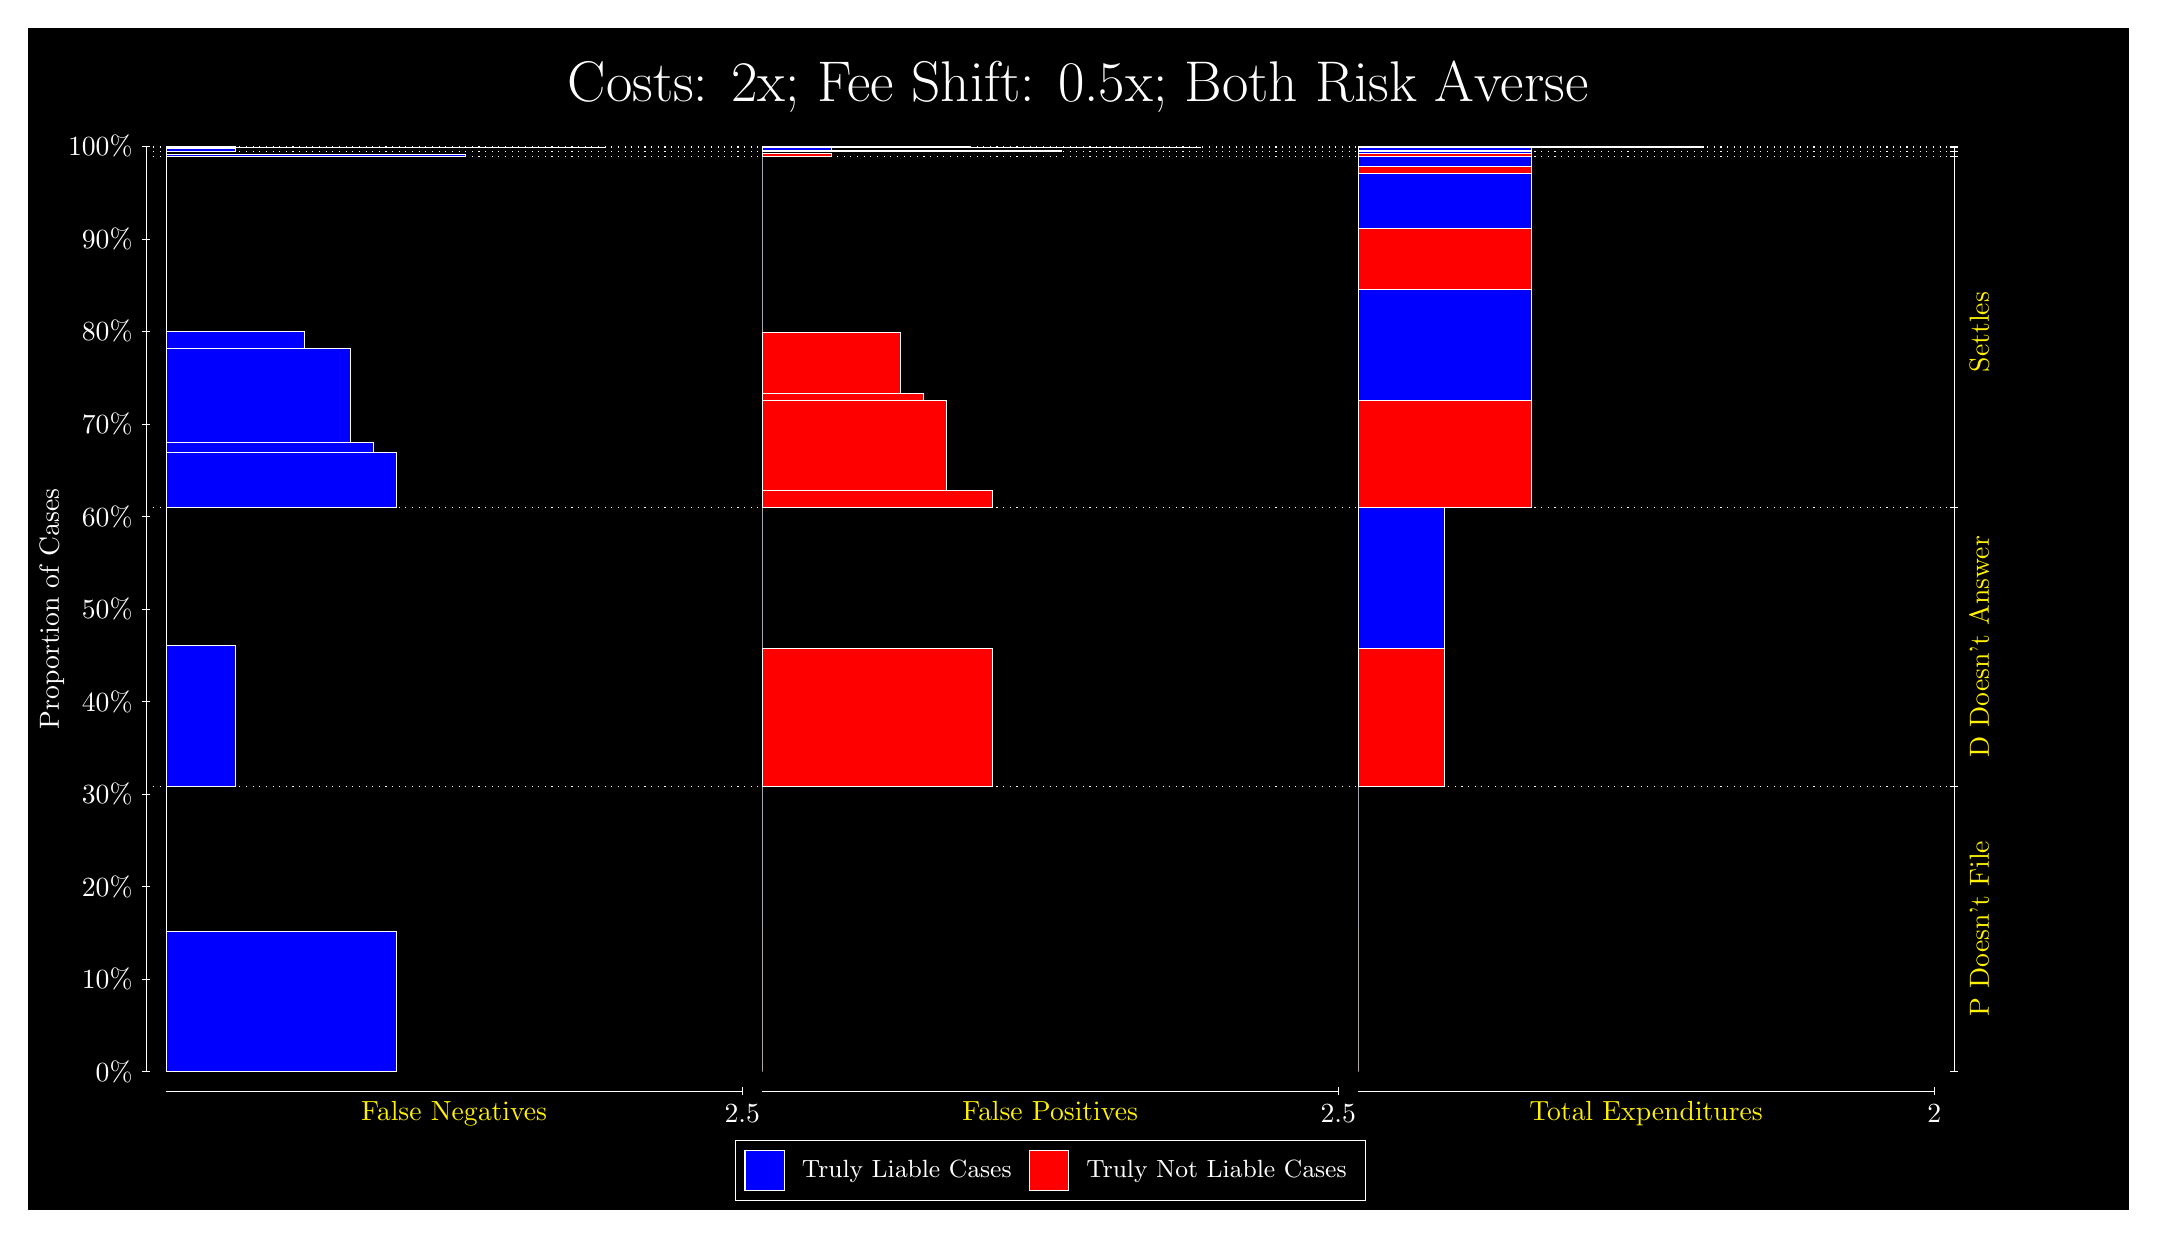
\begin{tikzpicture}
\draw[fill=black] (0,0) rectangle (26.667,15);
\draw[text=white] (0,13.5) rectangle (26.667,15) node[midway] {\huge Costs: 2x; Fee Shift: 0.5x; Both Risk Averse};
\draw[white, very thin] (1.5,1.75) -- (1.5,13.5);
\node[rotate=90, text=white, anchor=center] at (0.3, 7.625) {Proportion of Cases};
\draw[white, very thin] (1.45,1.75) -- (1.55,1.75);
\node[text=white, anchor=east] at (1.45, 1.75) {0\%};
\draw[white, very thin] (1.45,2.925) -- (1.55,2.925);
\node[text=white, anchor=east] at (1.45, 2.925) {10\%};
\draw[white, very thin] (1.45,4.1) -- (1.55,4.1);
\node[text=white, anchor=east] at (1.45, 4.1) {20\%};
\draw[white, very thin] (1.45,5.275) -- (1.55,5.275);
\node[text=white, anchor=east] at (1.45, 5.275) {30\%};
\draw[white, very thin] (1.45,6.45) -- (1.55,6.45);
\node[text=white, anchor=east] at (1.45, 6.45) {40\%};
\draw[white, very thin] (1.45,7.625) -- (1.55,7.625);
\node[text=white, anchor=east] at (1.45, 7.625) {50\%};
\draw[white, very thin] (1.45,8.8) -- (1.55,8.8);
\node[text=white, anchor=east] at (1.45, 8.8) {60\%};
\draw[white, very thin] (1.45,9.975) -- (1.55,9.975);
\node[text=white, anchor=east] at (1.45, 9.975) {70\%};
\draw[white, very thin] (1.45,11.15) -- (1.55,11.15);
\node[text=white, anchor=east] at (1.45, 11.15) {80\%};
\draw[white, very thin] (1.45,12.325) -- (1.55,12.325);
\node[text=white, anchor=east] at (1.45, 12.325) {90\%};
\draw[white, very thin] (1.45,13.5) -- (1.55,13.5);
\node[text=white, anchor=east] at (1.45, 13.5) {100\%};

\draw[white, very thin] (24.457,1.75) -- (24.457,13.5);
\draw[white, very thin] (24.407,1.75) -- (24.507,1.75);
\node[anchor=west] at (24.407, 1.75) {};
\draw[white, very thin] (24.407,5.374) -- (24.507,5.374);
\node[anchor=west] at (24.407, 5.374) {};
\draw[white, very thin] (24.407,8.9139) -- (24.507,8.9139);
\node[anchor=west] at (24.407, 8.9139) {};
\draw[white, very thin] (24.407,13.368) -- (24.507,13.368);
\node[anchor=west] at (24.407, 13.368) {};
\draw[white, very thin] (24.407,13.438) -- (24.507,13.438);
\node[anchor=west] at (24.407, 13.438) {};
\draw[white, very thin] (24.407,13.484) -- (24.507,13.484);
\node[anchor=west] at (24.407, 13.484) {};
\draw[white, very thin] (24.407,13.492) -- (24.507,13.492);
\node[anchor=west] at (24.407, 13.492) {};
\draw[white, very thin] (24.407,13.5) -- (24.507,13.5);
\node[anchor=west] at (24.407, 13.5) {};

\draw[white, very thin, fill=blue] (1.75,1.75) rectangle (4.6775,3.5367);
\draw[white, very thin, fill=red] (1.75,3.5367) rectangle (1.75,5.374);
\draw[white, very thin, fill=blue] (1.75,5.374) rectangle (2.6283,7.16);
\draw[white, very thin, fill=red] (1.75,7.16) rectangle (1.75,8.9139);
\draw[white, very thin, fill=blue] (1.75,8.9139) rectangle (4.6775,9.6183);
\draw[white, very thin, fill=blue] (1.75,9.6183) rectangle (4.3848,9.7401);
\draw[white, very thin, fill=blue] (1.75,9.7401) rectangle (4.092,10.93);
\draw[white, very thin, fill=blue] (1.75,10.93) rectangle (3.5065,11.147);
\draw[white, very thin, fill=red] (1.75,11.147) rectangle (1.75,13.368);
\draw[white, very thin, fill=blue] (1.75,13.368) rectangle (5.5558,13.395);
\draw[white, very thin, fill=red] (1.75,13.395) rectangle (1.75,13.438);
\draw[white, very thin, fill=blue] (1.75,13.438) rectangle (2.6283,13.471);
\draw[white, very thin, fill=red] (1.75,13.471) rectangle (1.75,13.484);
\draw[white, very thin, fill=blue] (1.75,13.484) rectangle (7.3123,13.487);
\draw[white, very thin, fill=red] (1.75,13.487) rectangle (1.75,13.492);
\draw[white, very thin, fill=blue] (1.75,13.492) rectangle (2.6283,13.497);
\draw[white, very thin, fill=red] (1.75,13.497) rectangle (1.75,13.5);
\draw[white, very thin, fill=red] (9.3189,1.75) rectangle (9.3189,3.5873);
\draw[white, very thin, fill=blue] (9.3189,3.5873) rectangle (9.3189,5.374);
\draw[white, very thin, fill=red] (9.3189,5.374) rectangle (12.246,7.1279);
\draw[white, very thin, fill=blue] (9.3189,7.1279) rectangle (9.3189,8.9139);
\draw[white, very thin, fill=red] (9.3189,8.9139) rectangle (12.246,9.1315);
\draw[white, very thin, fill=red] (9.3189,9.1315) rectangle (11.661,10.281);
\draw[white, very thin, fill=red] (9.3189,10.281) rectangle (11.368,10.37);
\draw[white, very thin, fill=red] (9.3189,10.37) rectangle (11.075,11.135);
\draw[white, very thin, fill=blue] (9.3189,11.135) rectangle (9.3189,13.368);
\draw[white, very thin, fill=red] (9.3189,13.368) rectangle (10.197,13.411);
\draw[white, very thin, fill=blue] (9.3189,13.411) rectangle (9.3189,13.438);
\draw[white, very thin, fill=red] (9.3189,13.438) rectangle (13.125,13.451);
\draw[white, very thin, fill=blue] (9.3189,13.451) rectangle (10.197,13.484);
\draw[white, very thin, fill=red] (9.3189,13.484) rectangle (10.197,13.488);
\draw[white, very thin, fill=blue] (9.3189,13.488) rectangle (9.3189,13.492);
\draw[white, very thin, fill=red] (9.3189,13.492) rectangle (14.881,13.494);
\draw[white, very thin, fill=blue] (9.3189,13.494) rectangle (11.954,13.5);
\draw[white, very thin, fill=red] (16.888,1.75) rectangle (16.888,3.5873);
\draw[white, very thin, fill=blue] (16.888,3.5873) rectangle (16.888,5.374);
\draw[white, very thin, fill=red] (16.888,5.374) rectangle (17.986,7.1279);
\draw[white, very thin, fill=blue] (16.888,7.1279) rectangle (17.986,8.9139);
\draw[white, very thin, fill=red] (16.888,8.9139) rectangle (19.083,10.281);
\draw[white, very thin, fill=blue] (16.888,10.281) rectangle (19.083,11.688);
\draw[white, very thin, fill=red] (16.888,11.688) rectangle (19.083,12.453);
\draw[white, very thin, fill=blue] (16.888,12.453) rectangle (19.083,13.157);
\draw[white, very thin, fill=red] (16.888,13.157) rectangle (19.083,13.246);
\draw[white, very thin, fill=blue] (16.888,13.246) rectangle (19.083,13.368);
\draw[white, very thin, fill=red] (16.888,13.368) rectangle (19.083,13.411);
\draw[white, very thin, fill=blue] (16.888,13.411) rectangle (19.083,13.438);
\draw[white, very thin, fill=red] (16.888,13.438) rectangle (19.083,13.451);
\draw[white, very thin, fill=blue] (16.888,13.451) rectangle (19.083,13.484);
\draw[white, very thin, fill=red] (16.888,13.484) rectangle (21.279,13.488);
\draw[white, very thin, fill=blue] (16.888,13.488) rectangle (21.279,13.492);
\draw[white, very thin, fill=red] (16.888,13.492) rectangle (21.279,13.494);
\draw[white, very thin, fill=blue] (16.888,13.494) rectangle (21.279,13.5);
\draw[white, dotted] (1.5,5.374) -- (24.457,5.374);
\draw[white, dotted] (1.5,8.9139) -- (24.457,8.9139);
\draw[white, dotted] (1.5,13.368) -- (24.457,13.368);
\draw[white, dotted] (1.5,13.438) -- (24.457,13.438);
\draw[white, dotted] (1.5,13.484) -- (24.457,13.484);
\draw[white, dotted] (1.5,13.492) -- (24.457,13.492);
\draw[white, very thin] (1.75,1.5) -- (9.0689,1.5);
\node[text=yellow, anchor=north] at (5.4094, 1.5) {False Negatives};
\draw[white, very thin] (9.0689,1.45) -- (9.0689,1.55);
\node[text=white, anchor=north] at (9.0689, 1.45) {2.5};

\draw[white, very thin] (9.3189,1.5) -- (16.638,1.5);
\node[text=yellow, anchor=north] at (12.978, 1.5) {False Positives};
\draw[white, very thin] (16.638,1.45) -- (16.638,1.55);
\node[text=white, anchor=north] at (16.638, 1.45) {2.5};

\draw[white, very thin] (16.888,1.5) -- (24.207,1.5);
\node[text=yellow, anchor=north] at (20.547, 1.5) {Total Expenditures};
\draw[white, very thin] (24.207,1.45) -- (24.207,1.55);
\node[text=white, anchor=north] at (24.207, 1.45) {2};

\node[text=yellow, centered, rotate=90] at (24.777, 3.562) {P Doesn't File};
\node[text=yellow, centered, rotate=90] at (24.777, 7.144) {D Doesn't Answer};
\node[text=yellow, centered, rotate=90] at (24.777, 11.141) {Settles};





\draw (12.978300999999998,1.5) node[draw=none] (baseCoordinate) {};
\begin{scope}[align=center]
        \matrix[scale=0.5, draw=white, below=0.5cm of baseCoordinate, nodes={draw}, column sep=0.1cm]{
            \node[rectangle, draw, minimum width=0.5cm, minimum height=0.5cm, fill=blue] {}; &
            \node[draw=none, font=\small, text=white] (B) {Truly Liable Cases}; &
            \node[rectangle, draw, minimum width=0.5cm, minimum height=0.5cm, fill=red] {}; &
            \node[draw=none, font=\small, text=white] (B) {Truly Not Liable Cases}; \\
            };
\end{scope}

\end{tikzpicture}
\end{document}